\chapter{Experimental Design}

In the our bouncing droplet system we observe surface waves guiding a droplet, and we're interested in learning more about the droplet-wave system in different settings. In this experiment, we will look at how features \textit{underneath} the surface of the oil (i.e. on the ``floor" of the tray) affect the motion of the droplet. 

A raised object on the floor of the tray (but still underneath the surface of the oil) can have an effect on height of the surface waves, and thus, on the motion of the walker\rf{tunneling}. Sometimes a droplet headed towards a raised object will be reflected backwards, as if from a collision with the object. For this reason, we refer to a raised object as a barrier. Oftentimes however, the droplet continues on and crosses the barrier without a collision, this is analagous to ``transmission" the quantum mechanical process of tunneling. In other words, for a given barrier we will see a probability of tunneling unique to that barrier. Other studies have shown that increasing barrier width decreases probability of tunneling\rf{tunneling}. This study looks at how height of the barrier affects the tunneling probability. 

To test the effect of a barrier's height on the probability of tunneling, I used a combination of procedures from the investigations of Bush\rf{pilot-wave}, Couder\rf{Couder2005}, and specifically, Eddi et al.\rf{tunneling}. These were slightly modified to fit some of the unique features of my experiment. In this section I aim to give some of the reasoning behind the tray design and data collection techniques, both of which are not well described in the literature.

\section{Setup}
    The cartoon of the setup is shown in \refFig{setup}, and a picture of the actual setup is shown in \refFig{group}(a). A waveform generator creates a sinusoidal signal which is amplified and fed into a shaker. The shaker vibrates the tray vertically. Both the frequency and the amplitude of the vertical oscillations can be controlled. 
    
    An accelerometer records the vertical acceleration of the tray and is read by an oscilloscope. A camera records the droplet as it bounces along the surface of the oil.  
    
   
    
\begin{figure}[h!]
	\centering
	\includegraphics[scale=0.8]{Setup.pdf}
	\caption{The experimental setup. The amplified signal from the wave generator drives the shaker. The accelerometer generates a signal which is read by the oscilloscope. The shield blocks disturbances to the experiment, while allowing the camera to document the trials.}
	\label{setup}
\end{figure}

\section{Materials}
The key components of this experiment are the shaker, the oil, and the tray. In this section I'll describe the specifics of the holy trinity, as well as some of the additional components used in data collection. 

\subsection{Tray}
The tray was made of plastic parts machined by the (MODEL NUMBER?) laser cutter. They were then glued together with GLUE?. The tray's design, which was based off of the tray in the tunneling experiment done by Eddi et al.\rf{tunneling}, naturally guides the droplet into a perpendicular collision with the barrier. The tray schematic is shown in \refFig{tray}. 

\begin{figure}[h!]
	\centering
	\includegraphics[scale=0.48]{Tray.pdf}
	\caption{The specifications of the tray design. The top view (left) highlights the main elements in the tray, while the cross section (right) illustrates the topography of the tray. Height is represented by the shading; darker shading is higher.}
	\label{tray}
\end{figure}

A thin layer of oil spills over the constraining rhombus shape. As long as the layer is thin enough, the droplet will remain in the rhombus container, but the waves will continue to propagate unimpeded. This gives the waves time to decay, and means that the droplets motion isn't chaotically affected by reflections of previous waves from the sidewalls, and is instead guided only by the unreflected waves. 

The rhombus shape serves to steer the droplet into a perpendicular collision with the barrier. This works because the droplet will pin-ball its way into the acute corner of the rhombus, and will shoot out in a straight line, directly towards the barrier as shown in \refFig{group}(c).

I designed my experiment to test barriers of three different heights: $2.75~\mathrm{mm}$, $3.0~\mathrm{mm}$, and $3.25~\mathrm{mm}$, measured from the bottom of the rhombus. A thin barrier of plastic made by the laser cutter has the tendency to bend and warp over time. The solution to this problem was to make these barriers taller than the specified heights, and create an cut-out in the rhombus so they could be inserted. The barrier cut-outs were deep enough to exactly counter the added height of the barrier, so the barriers still had (when measured from the surface of the rhombus) heights of $2.75~\mathrm{mm}$, $3.0~\mathrm{mm}$, and $3.25~\mathrm{mm}$. This also solved the problem of fixing the barriers in place, but still making them easily removable. These heights were chosen because they allowed for both passage over and blockage by the barriers. At the lowest heights, most droplets crossed over, whereas for taller barriers most droplets were blocked. 

The bottom of the tray was painted black in order to improve contrast, allowing the droplet to be more easily tracked by eye and by camera.

\begin{figure}
	\centering
	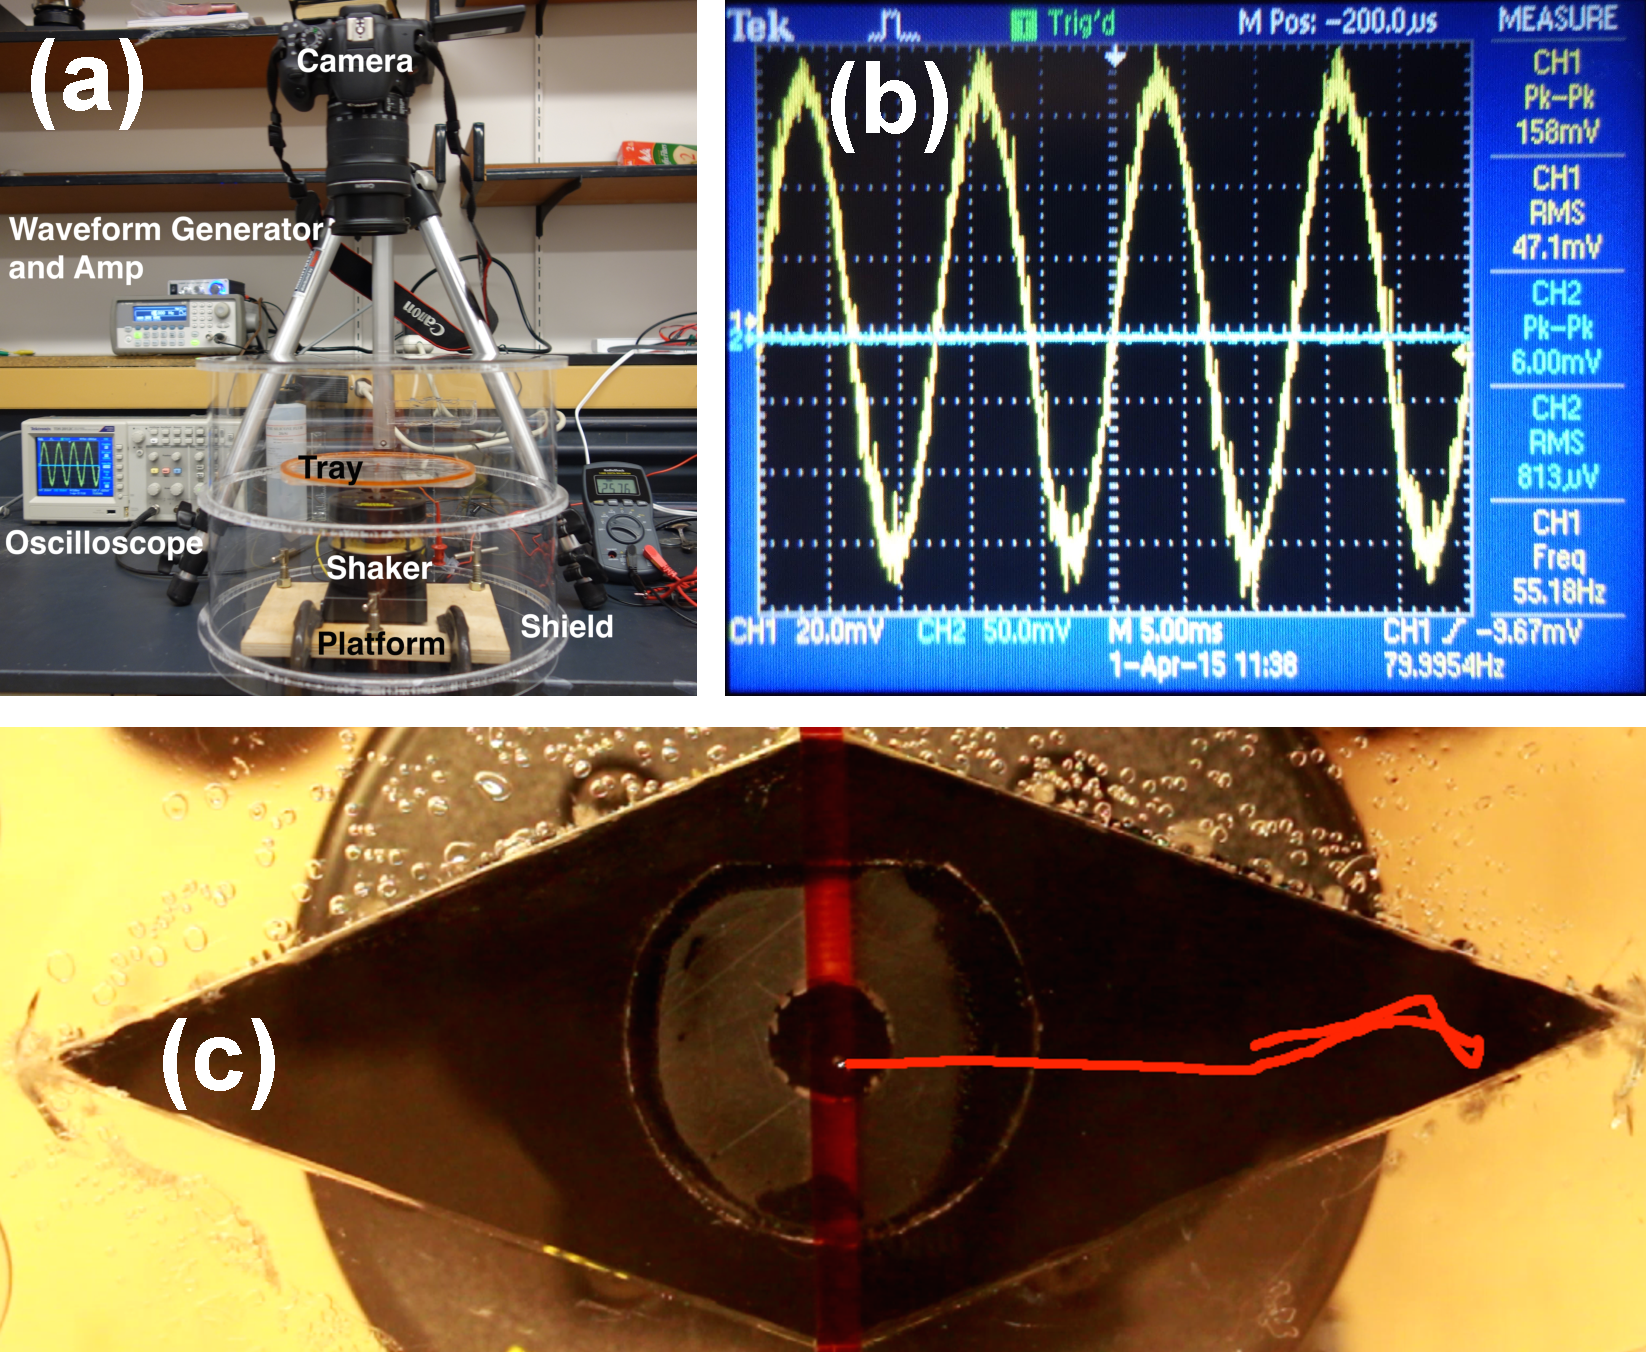
\includegraphics[scale=0.55]{group.pdf}
	\caption{(a)~The actual experimental setup. 
	(b)~The screen of the oscilloscope, showing the output from the accelerometer. The sine wave is the acceleration of the tray, and records a frequency $79.9954~\mathrm{Hz}$ and a peak to peak voltage of $158~\mathrm{mV}$. 
	(c)~A droplet of width $0.87~\mathrm{mm}$ walks into a corner and pinballs out into a straight line.}
	\label{group}
\end{figure}

\subsection{Silicon Oil}
    Silicon oil is the ideal choice of fluid for this experiment because it remains clean, it doesn't evaporate, and it can be purchased at specific viscosities. The silicone oil used in this experiment had a viscosity of 20 cSt (its viscosity is a little closer to water than olive oil) and was purchased from Clearco Products Co. Inc., Bensalem PA (CAS No: 63148-62-9). 20 cSt silicone oil, like the one used by Bush et al.\rf{pilot-wave} was chosen because it gives a larger walking regime\rf{pilot-wave} than more viscous oil, such as the 50 cSt viscosity oil used by Couder\rf{Protiere2005}. The tray requires about $20~\mathrm{mL}$ of fluid.
    
    It is of vital importance to keep the oil as clean as possible because it keeps the droplet bouncing for longer. This means protecting from particulate matter that is already in the tray. Contamination can be minimized by cleaning the tray before pouring the oil in.
    
\subsection{Shaker}
    To shake the tray, we used a mechanical wave driver made by Pasco Scientific, Roseville CA, model SF-9324. This shaker was designed to drive a string or an elastic cord, not a $200$ gram tray with oil inside, which was probably at the limit of what the shaker can handle. 

\subsection{Waveform Generator and Amplifier}
    The shaker was driven with the Agilent Arbitrary Waveform Generator model 33210, which was controlled digitally and thus created waves of a constistent frequency. The waveform generator was usually set to produce a sine wave of $80~\mathrm{Hz}$. Adding a Lepai LP2020A+ digital amplifier to the wavefunction generator meant the amplitude of the tray could be precisely controlled. This signal, which was also measured with a multimeter, was then fed into the shaker.    
            
\subsection{Accelerometer}  
    Knowing the tray's acceleration allows us to characterize the behavior of our system. To measure acceleration, we attached an ADLX 326 triple axis accelerometer (made by Adafruit, New York City NY) to the bottom of the tray. The method of attachment was screws, since it provided a much more firm hold than tape or glue while allowing for removal. The accelerometer has a range of $\pm$16$g$, perfect for measuring the accelerations in our setup, usually below $5g$'s. 
      
      The signal from the z-axis of the accelerometer was output directly into the oscilloscope, a sample output can be seen in \refFig{group}(b). For the vibrating tray, the output was approximately sinusoidal (as expected). The spec sheet for the accelerometer indicates that the sensitivity can be translated to $57 \pm 6~\mathrm{mV/g}$. 
    
\subsection{Shield}
    A large, see-through cylinder (covered at one end) was manufactured using the laser cutter. When placed over the tray, it served the purpose of keeping the oil clean from particulate matter and preventing wind currents from influencing the motion of the walker.       
   
\subsection{Leveling Platform}
    A leveling platform was made out of wood supports the shaker. Three adjusters allowed for precise adjustment of tilt. The tray was tuned using a level placed inside the tray (before the oil was added). 

\subsection{Camera}       
 
To document trials, a Sony RX100 camera supported by a tripod aimed directly down at the tray. 

\section{Procedure}
Once the exact walking parameters are established (frequency and driving amplitude), tunneling measurements and a few different barrier heights can be made. 

\subsection{Finding the Walking Regime}

Before investigating the rate of tunneling using different barriers, a rough estimate of the walking regime at a frequency of $80~\mathrm{Hz}$ must be made. A ``map" similar to the one in \refFig{regime} will be sketched out, but rather than looking at all of the different kinds of bouncing we will limit ourselves to only the walking regime. Reproducing this figure allows us to find the parameters that are specific to our unique setup, which could have slightly different height, tray, oil, and shaker configurations than those used in the literature. 

Droplet size is measured using a recorded video of the walking droplet in motion. By comparing the number of pixels making up the diameter of the droplet (unknown measurement) to the number of pixels making up the diameter of the tray (known measurement), we can estimate the length associated with  each pixel, and thus find the diameter of the droplet in centimeters. 

Driving acceleration values are measured by the accelerometer and displayed on the oscilloscope. 

To ensure that every trial has the same oil depth, we must measure the volume of the oil before filling the tray. Knowing the volume of the tray and of each barrier, we can get a value for the oil depth without interfering with the system. In this way, oil height can be kept constant.

\subsection{The Experiment}

Tunneling was examined for three different barrier heights. At each height (and at a constant frequency of 80 Hz and constant driving acceleration), a string of continuous collisions were filmed with the camera. From this data, a basic tunneling probability was calculated, which provides the most simplistic analysis of this system. 

The tray is designed such that most of the droplet's collisions with the barrier occur ``head on" (i.e. perpendicular to the length of the barrier), but not all collisions unfold ideally. A more involved analysis in \textit{Tracker} requires looking at the component of velocity of the droplet perpendicular to the length of the barrier, and determining the probability of tunneling given this value. Since not all collisions in the simplistic analysis occur at the same velocity, this method allows for a more methodical analysis of the phenomena. 
